\subsection{Model Diagnostics}
By using a linear regression model for calculating the loss and gain $\beta $ 
values in the neural (BOLD) signals, we have made the following underlying 
assumptions:
\begin{enumerate}
    \item Normailty of errors
    \item Homoscedasticity (constant variance) or errors  
    \item Linearity of relationship between the explanatory and response
    \item Statistical independence of errors   
    \item All voxels and all subjects follow the same linear model. 
\end{enumerate}
The first four assumption can be motivated by using the residuals as a proxy
for the errors since the errors are unobservable. Here we check the first 
three assumptions by following the standard regression diagnostics plots and 
analysis. The fourth condition, checking for independence of errors, is 
equivalent to checking that no correlation exists between consecutive errors 
in our time serires structure. A simple explanation is given in 
\textit{Simplifications of Model}, so it is leaved out here. For the fifth 
assumption, it may that there are some observations/conditions that do not 
obey the linear model. The methods used to detect these usual observations is 
further discussed in \textit{Outlier Detection}, so it will be left out here. 

\subsubsection{Linearity and Constant Variance}
The residual versus fitted values plot \ref{fig:residual_vs_fitted} is a 
standard plot for observing constant variance of errors and potential deviations
from linearity

\begin{figure}[ht]
\centering
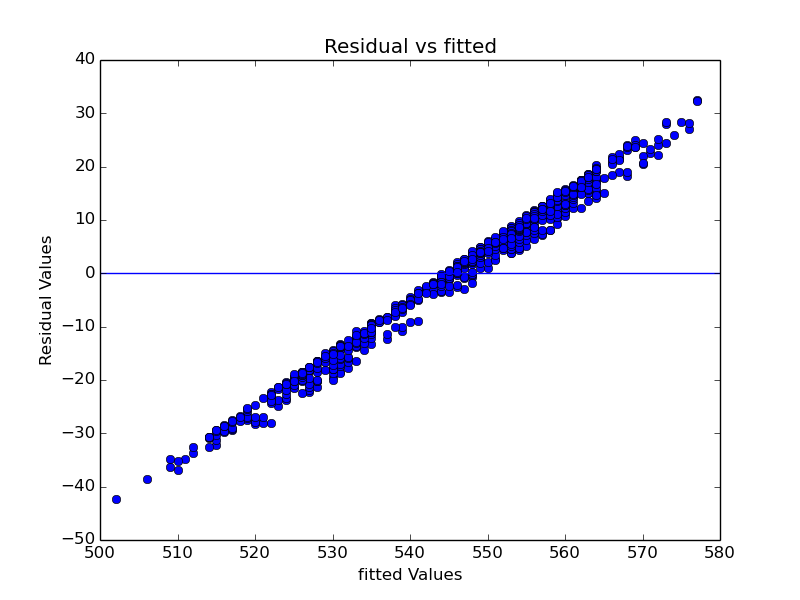
\includegraphics[scale=0.5]{figures/res_fittedval}  
\caption{Residual vs Fitted Values for voxel 40000 across time}
\label{fig:residual_vs_fitted}
\end{figure}

From the figure we can see there is clear linear pattern to residual. The
residuals seems to increase as the fitted values increase, suggesting a 
variance-stabilizing transformation to the response vector. We will keep this 
in mind in out future analysis. 

\subsubsection{Normality}
Normality of the errors is checked by checking the normality of the residuals. 
The normal qq-plot (Quantile-Quantile Plot) \ref{fig:qqplot} shows quantiles
of the sorted residuals averaged across time against the normal theoretical 
quantiles. Ideally, the relationship should be linear. Here we show the qqplot
of the quantiles of residuals for the 40000th voxel, taken as a random voxel 
near the center of the image. We can see that the normality assumption is 
reasonable. In practice, this makes sense because we expect the accross-time
changes/errors of estimates for a sigle voxel to be close to normally 
distributed.

\begin{figure}[ht]
\centering
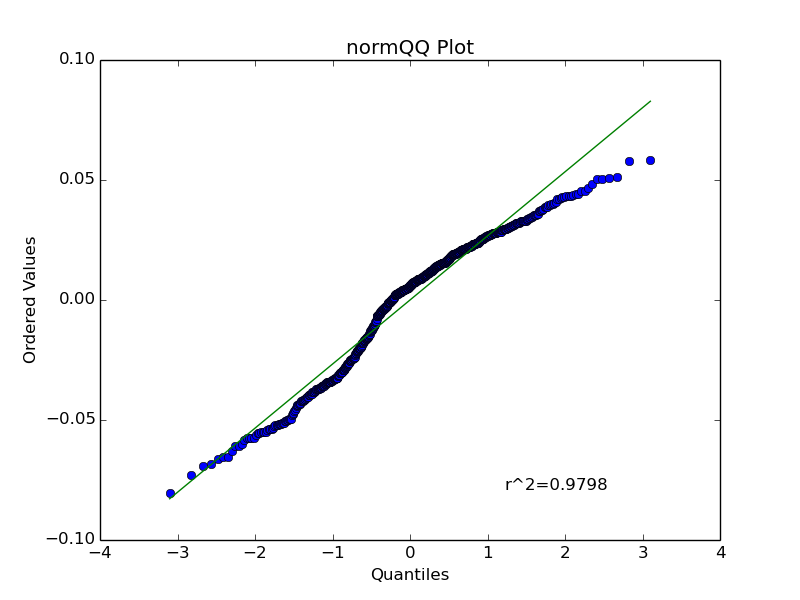
\includegraphics[scale=0.5]{figures/qqplot}  
\caption{Normal QQ plot of the residuals for 40000 th voxel.}
\label{fig:qqplot}
\end{figure}



